%!TEX root = ../../master.tex
\section{The Model}\label{sec:themodel}
This section will showcase the model made to express the design from \myref{cha:Design}.
For simplicity the the model in this chapter has been split into two parts, an initializing phase and the main loop.
Before the template is shown the code for the system will be presented.
The template has local code which can be seen on \myref{device_local}.
This code contains functions which encapsulate many updates from the template, which would otherwise clutter the template with too many specifics.

\begin{lstlisting}[style=UPPAAL,
caption={Local code for Device.}, label={device_local}, multicols=2]
// Place local declarations here.
clock x;
clock transmit_time;
int k = -1;                     //Timeslot
bool Connected = false;

// Local copies of globals
// Number of devices connected
int local_n = 0; 
// Current time slot in the frame
int local_i = 0;

void increment_Slot(){
    local_i = (local_i % local_n)+1;
}

void receive()
{
    local_i = i;
    local_n = n;
}

void join_Network(){
    k=n;
    n = n+1;
    local_n = local_n+1;
    Connected = true;
    Connected_Counter++;
}

void create_Network(){
    i = 0;
    n = 2;
    k = 1;
    local_i = 0;
    local_n = 2;
    Connected_Counter = 1;
    Connected = true;
    x:=0;
}

void make_Payload(){
    i = local_i;
    n = local_n;
}

\end{lstlisting}

The global code for the system can be seen on \myref{uppaal_Global}.
This is where the system sends information from one device to another, when one device transmit it will change the global values, while the receiving devices will get the global values and put them locally.
Another important thing to note is the broadcast channel transmit, which will be used as descibred in \myref{UPPAAL_Models}.

\begin{lstlisting}[style=UPPAAL,
caption={Code for the global declarations.}, label={uppaal_Global}, multicols=2]
// Place global declarations here.
// Number of Timeslots connected
int n = 0;         
// Current time slot in the frame
int i = 0;            
//Global Counter for Connected Devices                    
int Connected_Counter = 0;
//Timeslot Length
const int Delta = 250;                 
const int Delta_Proc = Delta/5;
const int Real_Tx_Time = Delta/2;
const int Tx_Time = Delta_Proc + Real_Tx_Time;
const int Initial_Wait_Time = Delta*3;
int Startup_Time = Initial_Wait_Time*2;
clock startup;

//Channel
broadcast chan transmit;

//Device Creation
const int N = 4;
typedef int[1,N] id_t;
\end{lstlisting}

Finally to instantiate the system, a system declaration is needed which can be seen on \myref{UPPAAL_System_Dcl}.
This creates $N$ devices each with a unique ID from $1 - N$ because of the code seen on \myref{uppaal_Global}, at the comment Device Creation.

\begin{lstlisting}[style=UPPAAL,
caption={Code for system declarations.}, label={UPPAAL_System_Dcl}]
system Device;
\end{lstlisting}

\begin{figure}
  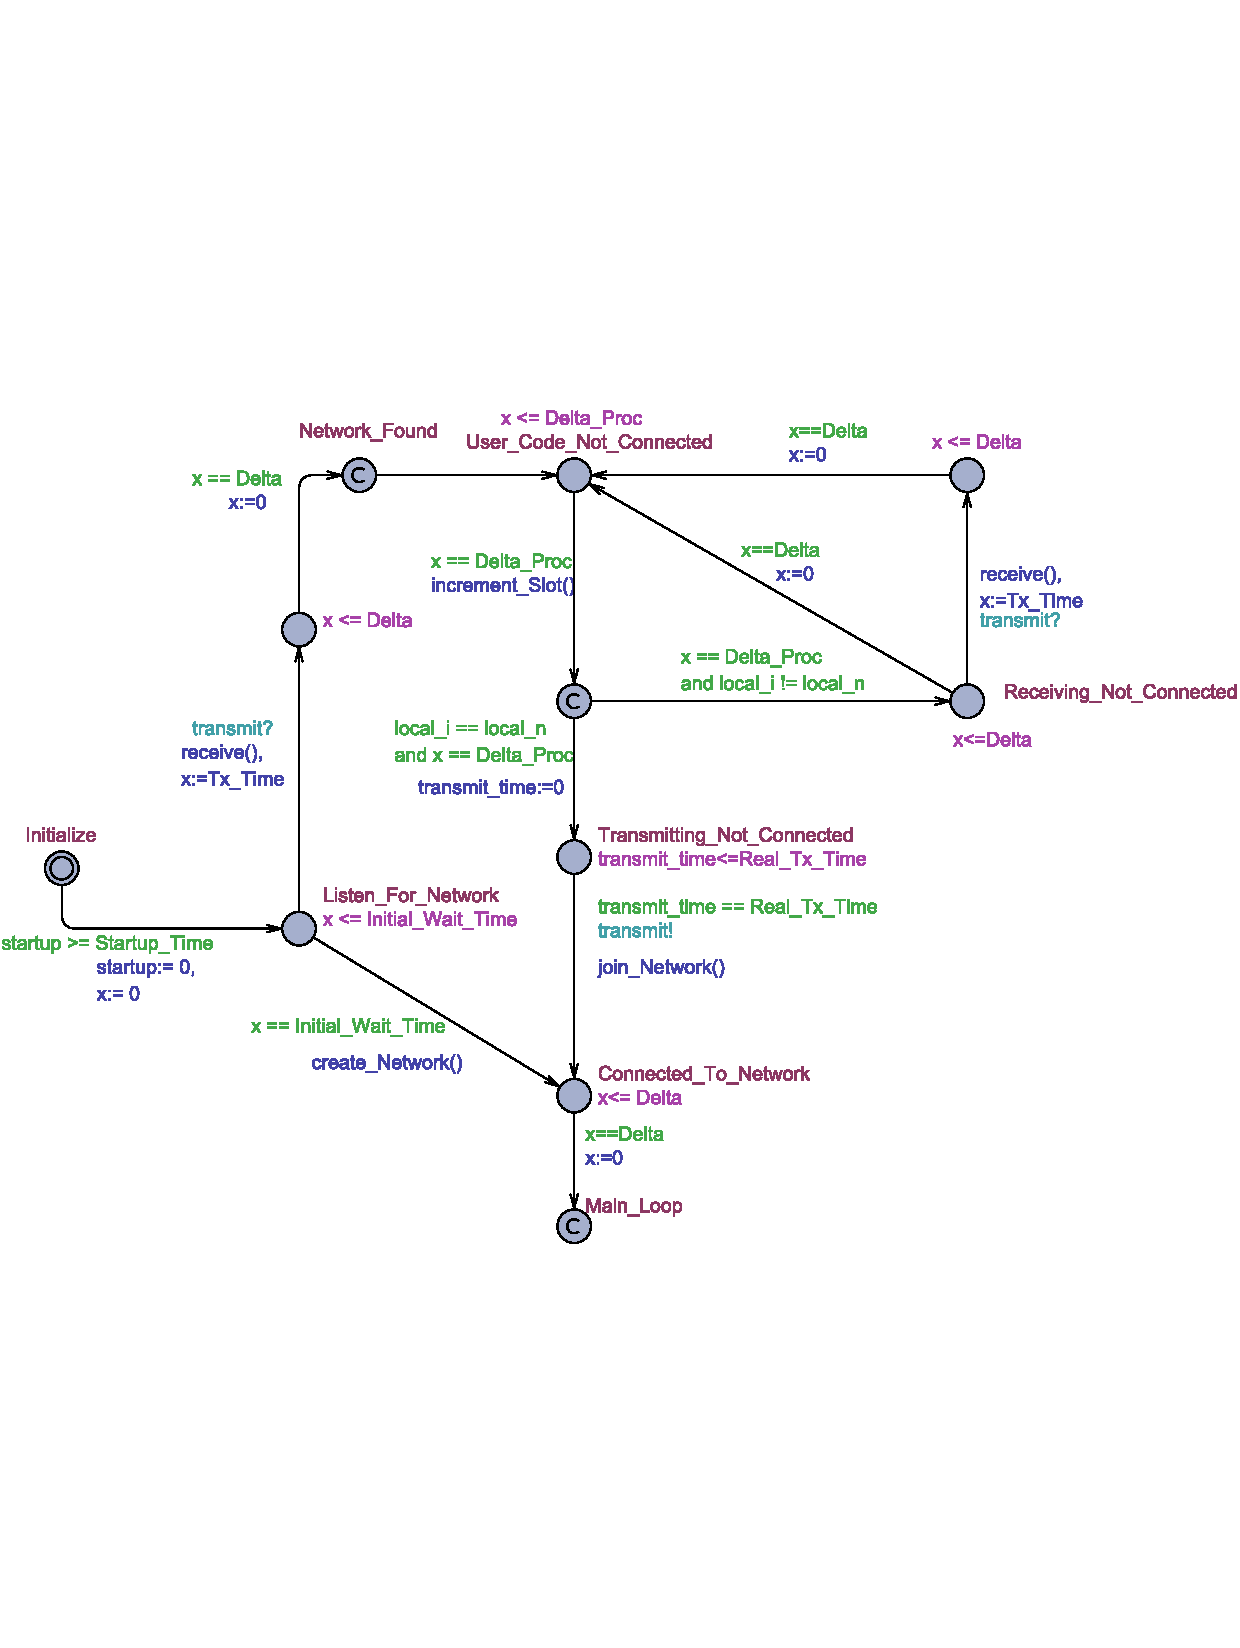
\includegraphics[width=1\textwidth]{Figures/Model/Device_Connecting.pdf} 
\caption{UPPAAL Model showing how the devices initialize.}
\label{fig:UPPAAL_Intitialization}
\end{figure}

\bigskip \noindent
The first part to be presented of the template will be the initialization, which can be seen on \myref{fig:UPPAAL_Intitialization}.
The initial location has a clock \texttt{startup}, which makes sure that devices will leave the initial location one at a time.
When one of the devices leave this location, \texttt{startup} will reset, and another will leave the location when \texttt{startup} once again reaches the desired time.
It should be mentioned that this \texttt{Startup\_Time} is proportional with the number of devices in the system.
This is because when the frame of the network grows, \texttt{Startup\_Time} must match the increase in frame length such that only one device can be released per frame.

With the current values in the model creating a network with at least six devices is doable, it has not been tested with more.
While the other devices are waiting to be released, the device which was the first to leave will listen for a network, as there is obviously no network yet the device will fire the edge towards the \texttt{Connected\_To\_Network} location.
The device will setup the initial values for the network, change its boolean \texttt{Connected} to true, this all happens in the function \texttt{create\_Network()}. The device will move onwards towards the main loop, which will be shown later.
When the next device leaves the initial location it will successfully find a network as one was just created; in doing so the device will fire the edge the other edge, where the broadcast channel \texttt{transmit} is seen.
The device will stay in this location until the communication phase of the time-slot is complete, and then it will continue towards the committed location \texttt{Network\_Found} and reset the clock \texttt{x} to zero.
This location is committed as its purpose is simply visual working as a context switch between having found a network and entering the loop to wait for the empty-slot.
When it has just received a transmission, the device which just transmitted will according to \myref{cha:Design} be performing user code, and therefore the device trying to connect should be waiting for the next time-slot so the other devices are ready to receive again.

\bigskip \noindent
When \texttt{x} is equal to \texttt{Delta\_Proc}, the time designated to perform user code, the device will fire the edge to the committed location directly under \texttt{User\_Code\_Not\_Connected} once again.
In this location when \texttt{x} is not zero, the device checks whether \texttt{i}, the current time-slot, is the empty-time slot, if it is the device will transmit and ultimately connect to the network increasing the number of time-slots in the network according to the specifications in \myref{cha:Design}.
If the empty slot was not the current time-slot, the device will instead go to the location \texttt{Receiving\_Not\_Connected} where it will receive the other devices' transmissions, once again reset \texttt{x} to zero and loop until eventually the empty-slot occurs, where it will connect to the network.
The model can be seen on \myref{fig:UPPAAL_Connected}.

\begin{figure}
  
\includegraphics[width=1\textwidth]{Figures/Model/Device_Connected.pdf} 
\caption{UPPAAL Model showing the devices' main loop.}
\label{fig:UPPAAL_Connected}
\end{figure}

When a device has been connected to a network it will instantly move to the location main loop, where it will perform the actions as described in the pseudocode of \myref{cha:Design}.

First it moves to a location \texttt{User\_Code} where it will perform user code until the the clock \texttt{x} is equal to \texttt{Delta\_Proc}.
As soon as this is the case the device will move on to a committed location where it will choose to either transmit or receive depending on whether or not the current time-slot belongs to the device or not.
When a device has transmitted a transmission, it will move to a waiting location where it will wait until the time-slot has officially ended, which is when the clock \texttt{x} is equal to \texttt{Delta}, reset the clock \texttt{x} and then it will execute the main loop once again.
This also happens when the device in the emptyslot is transmitting, the device waits before starting the main loop.
When the device is in the location \texttt{Receiving}, if nothing has been transmitted and the clock \texttt{x} is equal to \texttt{Delta} the device will go increment its \texttt{i\_local} value reset the clock \texttt{x} and restart the main loop. 
This case happens whenever the empty slot is the current time-slot and no new device is trying to connect to the network.
According to the specification of \myref{cha:Design} devices which receive a transmission will synchronize to the clock of the transmitting device, this is implemented in the system as the update \texttt{x:=Tx\_Time}, where \texttt{Tx\_Time} is the sum of \texttt{Delta\_Proc} and \texttt{Real\_Tx\_Time}, so it is the time the transmitting device has spent until it is done transmitting.
A function to calculate this synchronized time will be require to implement the model on an Arduino.

\section{Verifying the Model}\label{sec:verifyingTheModel}

As mentioned in \myref{subsec:uppaal} it is possible to make queries to verify that some given properties are true.
\myref{sec:Pseudo} contains statements which should be true for a correctly connected network.
These statements can be written as queries in UPPAAL, which the tool will then determine to be correct or not. 
The queries described here have been tested with a system consisting of up to 6 devices, but it is recommended to go no higher than 4 in one system as the queries computation time increase dramatically.
The queries for the system will be given one by one with along with a description of what they represent.
\begin{lstlisting}[style=UPPAAL, title={This query requires that eventually if all devices are connected, then no pair of devices have the same \texttt{k}, unless the pair consists of the same two devices.}]
1. A<> forall(i : id_t) forall(j : id_t) Device(i).Connected and
         Device(j).Connected and Device(i).k == Device(j).k imply i == j
\end{lstlisting}

\begin{lstlisting}[style=UPPAAL, title={The query requires that there is no deadlock in the system.}]
2. A[] not deadlock
\end{lstlisting}

\todo[inline]{The following query should cover ALL transmitting states.}
\begin{lstlisting}[style=UPPAAL, title={This query requires that no pair of devices are in the ``Transmitting'' state at the same time.}]
3. A[] forall(i : id_t) forall(j : id_t) 
      ((Device(i).Transmitting and Device(j).Transmitting) 
    or (Device(i).Transmitting and Device(j).Transmitting_Not_Connected) 
    or (Device(i).Transmitting_Not_Connected and Device(j).Transmitting_Not_Connected)) 
    imply i==j
\end{lstlisting}
\begin{lstlisting}[style=UPPAAL, title={This query requires that if two devices are both in the location \texttt{User\_Code} they then have the same value of their \texttt{local\_i}}. This imply that they are synchronised.]
4. A[] forall(i : id_t) forall(j : id_t) Device(i).User_Code and 
        Device(j).User_Code imply Device(i).local_i == Device(j).local_i
\end{lstlisting}
\begin{lstlisting}[style=UPPAAL, title={This query requires that if a device \texttt{i} and a device \texttt{j} is both connected, they then have the same value of their \texttt{local\_n}. If they were different it would mean that they are not in the same network, and as such would have different numbers of time-slots in their networks. But the system model makes sure that this is not the case.}]
5. A[] forall(i : id_t) forall(j : id_t) 
    Device(i).Connected and Device(j).Connected 
    imply Device(i).local_n == Device(j).local_n
\end{lstlisting}

\begin{lstlisting}[style=UPPAAL, title={This query requires that if it is always true that all devices never has the the time-slot which one of the devices has locally as the empty-slot. If any device did have this, it would mean that a device was out of sync, since it did not know which time-slot would be the empty one. }]
6. A[] forall(i : id_t) forall(j : id_t) Device(i).k != Device(j).local_n
\end{lstlisting}

\begin{lstlisting}[style=UPPAAL, title={This query requires that if a device is connected it has a \texttt{k} value between \texttt{0} and \texttt{n}, which is the number of time-slots in the frame}]
7. A[] forall(i : id_t) 
    Device(i).Connected and Device(j).Connected 
    imply Device(i).k < n and Device(i).k > 0
\end{lstlisting}

\begin{lstlisting}[style=UPPAAL, title={The query requires that if a device is connected, is it then true that the number of devices connected to a network is equal to one less the number of time-slots in the frame of a network. }]
8. A[] forall(i : id_t) Device(i).Connected imply Connected_Counter == n-1
\end{lstlisting}

All of these queries will yield a true result when run with 6 devices on the model presented in this chapter.
Note that queries have been added to verify the model beyond the ones derived from the statements in \myref{sec:Pseudo}, an example is query 2.

The queries 1, 7 and 8 together make up the statement (e) from \myref{sec:Pseudo}, since if no devices have the same time-slot k and if the number of devices is one less than the number of time-slots and all time-slots in the range $[1, N-1]$ corresponds to an occupied time-slot in the network.

Since all of these statements hold true, it is concluded that the model does indeed do what it was designed to do, and an implementation according to the specification should theoretically work and be possible to create.
